\section{Double Sided Tetrahedron}
Another shape that we considered exploring was the triangular bipyramid or double sided tetrahedron. This shape is interesting because (since all the faces are triangles) it has the minimum number of vertices required to reach six faces at just five vertices, compared to a cuboid which has eight vertices. However, we chose not to explore this figure for two reasons:\\
\begin{itemize}
    \item A pyramidal shape is easier to make in such a way that one face has a very high probability, since it has a base.\\
    \item Our analysis for six sided pyramidal shapes could be easily extended to five sided pyramidal shapes, while a triangular bipyramid would require a completely independent analysis.\\
\end{itemize}
\begin{figure}[h]
\center
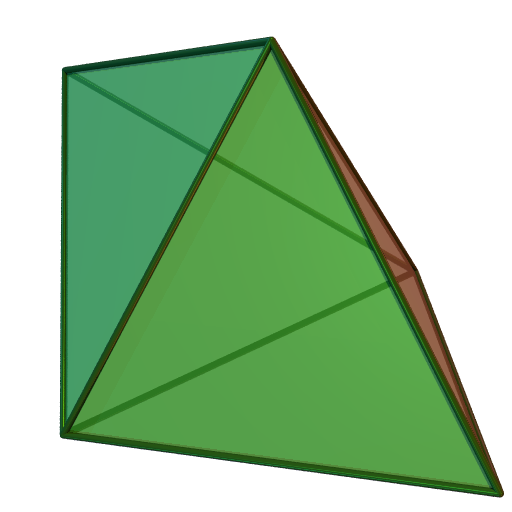
\includegraphics[scale=0.6]{DStetra.png}
\caption{}
\label{fig:DStetra}
\end{figure}